   
   \section{Data Packing and Unpacking}

   \begin{frame}
      \frametitle{Data Packing and Unpacking}
      \begin{center}
      \Huge{Data Packing and Unpacking}
      \end{center}
   \end{frame}
   
   \begin{frame}
      \frametitle{Data Packing and Unpacking}
      \begin{itemize}
         \item TrickHLA supports a data packing and unpacking mechanism so that
         data transformations can be applied to the data before being sent to
         (pack) or after received from (unpack) another federate.
         \item For example, your simulation uses a phase variable in radians but
         the FOM specifies the phase variable  will be exchanged between
         federates in degrees.
         \item Packing/unpacking is added to your simulation by extending the
         \texttt{TrickHLAPacking} class and implementing the \texttt{pack()}
         and \texttt{unpack()} functions.
         \item TrickHLA will automatically call your \texttt{pack()} and
         \texttt{unpack()}
         functions at the appropriate time.
         \item Adding packing/unpacking to your simulation consists of three
         steps \textellipsis
      \end{itemize}
   \end{frame}

   \begin{frame}[fragile]
      \frametitle{Data Packing and Unpacking}
      \framesubtitle{Step 1: Extending the \texttt{TrickHLA::Packing} Class - \texttt{SinePacking.hh}}
      \begin{itemize}
         \item Step 1: Extend the \texttt{TrickHLA::Packing} class and implement
         the \texttt{pack()} and \texttt{unpack()} functions in \texttt{SinePacking.hh} :
      \end{itemize}
\begin{Verbatim}[frame=single, fontsize=\tiny]
   #include SineData.hh
   #include "TrickHLA/include/TrickHLAPacking.hh"

   class SinePacking : public TrickHLAPacking
   {
     public:
      // Initialize the packing object.
      void initialize( SineData * sim_data );
      // From the TrickHLAPacking class.
      virtual void initialize_callback( TrickHLAObject * obj );

      // From the TrickHLAPacking class.
      virtual void pack();
      // From the TrickHLAPacking class.
      virtual void unpack();

     private:
      SineData * sim_data; // -- Simulation data.
      double phase_deg;    // d  Phase offset in degrees.
   };
\end{Verbatim}
   \end{frame}

   \begin{frame}[fragile]
      \frametitle{Data Packing and Unpacking}
      \framesubtitle{Step 1: Extending the \texttt{TrickHLA::Packing} Class - \texttt{SinePacking.cpp}}
      \begin{itemize}
         \item Example in \texttt{SinePacking.cpp} :
      \end{itemize}
\begin{Verbatim}[frame=single, fontsize=\scriptsize]
void SinePacking::initialize( // RETURN: -- None.
      SineData * sim_data)    // IN:     -- Simulation data.
{
   this->sim_data = sim_data;
}
void SinePacking::pack()    // RETURN: -- None.
{
   // For this example to show how to use the Packing API's, we
   // will assume that the phase shared between federates is in
   // degrees so convert it from radians to degrees.
   phase_deg = sim_data->get_phase() * 180.0 / M_PI;
}
void SinePacking::unpack()  // RETURN: -- None.
{
   // For this example to show how to use the Packing API's, we
   // will assume that the phase shared between federates is in
   // degrees so convert it back from degrees to radians.
   sim_data->set_phase( phase_deg * M_PI / 180.0 );
}
\end{Verbatim}
   \end{frame}

   \begin{frame}[fragile]
      \frametitle{Data Packing and Unpacking}
      \framesubtitle{Step 2: Add Packing Object to \texttt{S\_define}}
      \begin{itemize}
         \item Step 2: In the \texttt{S\_define} file add your packing object
         to each simulation object that needs to have its data packed/unpacked.
         \item Make sure to initialize your packing object if it needs it.
      \end{itemize}
\begin{Verbatim}[frame=single, fontsize=\tiny]
   class ASimObject : public Trick::SimObject {
      …
      SineData     sim_data;
      SinePacking  packing;

      ASimObject() {
        P50 ("initialization") packing.initialize( &sim_data );
        …
      }
   };

   class PSimObject : public Trick::SimObject {
      …
      SineData     sim_data;
      SinePacking  packing;

      PSimObject() {
        P50 ("initialization") packing.initialize( &sim_data );
        …
      }
   };
\end{Verbatim}
   \end{frame}

   \begin{frame}[fragile]
      \frametitle{Data Packing and Unpacking}
      \framesubtitle{Step 3: Configuration}
      \begin{itemize}
         \item Step 3: Configure the data object in the input.py file to use
         your packing object by setting the data object’s packing field. For
         example in the \texttt{RUN\_a\_side/input.py} file:
\begin{Verbatim}[frame=single, fontsize=\scriptsize]
THLA.manager.objects[0].packing = A.packing
THLA.manager.objects[1].packing = P.packing
\end{Verbatim}
         \item Don’t forget to update the attribute \texttt{trick\_name} field
         to use the correct Trick simulation variable (i.e. the transformed
         data from the \texttt{pack()} and \texttt{unpack()} functions).
   To use the simulation data phase in radians:
\begin{Verbatim}[frame=single, fontsize=\scriptsize]
THLA.manager.objects[0].attributes[3].trick_name = "A.sim_data.phase”
THLA.manager.objects[1].attributes[3].trick_name = “P.sim_data.phase”
\end{Verbatim}
         \item To use the transformed phase in degrees to be shared with the
         other federates:
\begin{Verbatim}[frame=single, fontsize=\scriptsize]
THLA.manager.objects[0].attributes[3].trick_name = "A.packing.phase_deg”
THLA.manager.objects[1].attributes[3].trick_name = “P.packing.phase_deg”
\end{Verbatim}
      \end{itemize}
   \end{frame}

   \begin{frame}
      \frametitle{Data Packing and Unpacking}
      \framesubtitle{TrickHLA jobs in THLA.sm}
      \begin{figure}
      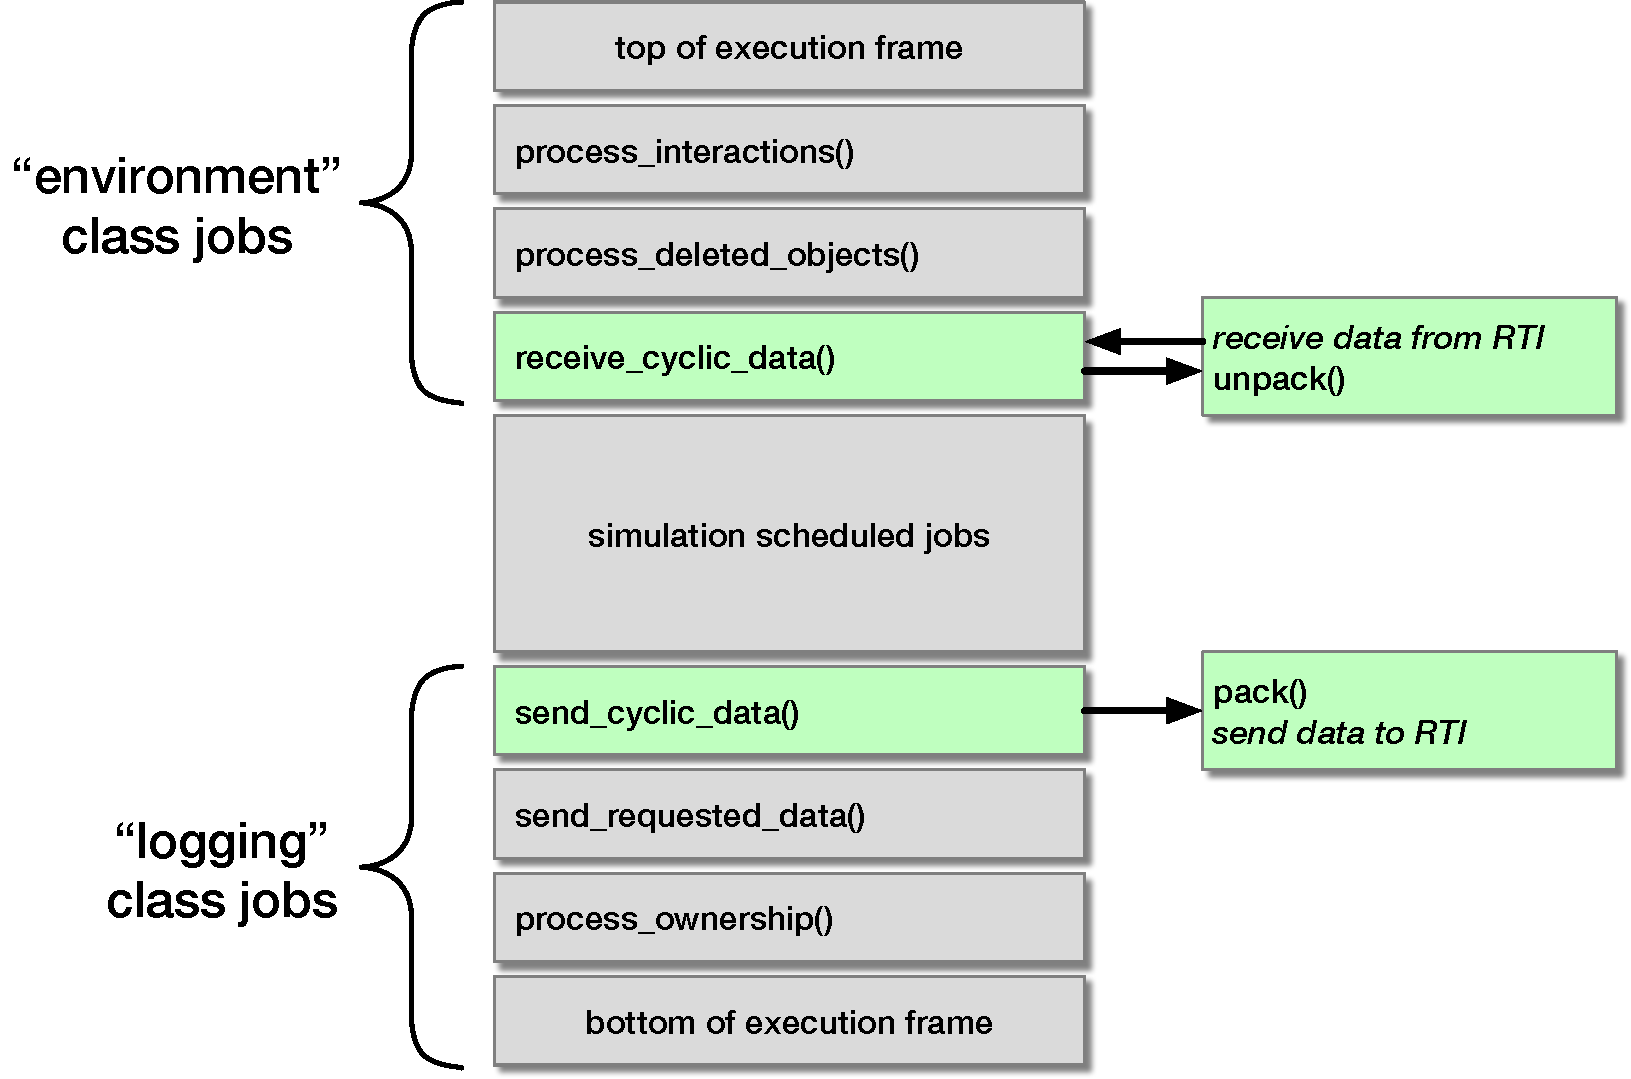
\includegraphics[scale=0.4]{TutorialTHLAPackingJobs.pdf}
      \end{figure}
   \end{frame}